
\section*{Общая характеристика работы}

\newcommand{\actuality}{\underline{\textbf{\actualityTXT}}}
\newcommand{\progress}{\underline{\textbf{\progressTXT}}}
\newcommand{\aim}{\underline{{\textbf\aimTXT}}}
\newcommand{\tasks}{\underline{\textbf{\tasksTXT}}}
\newcommand{\novelty}{\underline{\textbf{\noveltyTXT}}}
\newcommand{\influence}{\underline{\textbf{\influenceTXT}}}
\newcommand{\methods}{\underline{\textbf{\methodsTXT}}}
\newcommand{\defpositions}{\underline{\textbf{\defpositionsTXT}}}
\newcommand{\reliability}{\underline{\textbf{\reliabilityTXT}}}
\newcommand{\probation}{\underline{\textbf{\probationTXT}}}
\newcommand{\contribution}{\underline{\textbf{\contributionTXT}}}
\newcommand{\publications}{\underline{\textbf{\publicationsTXT}}}


{\actuality} Круг задач, решаемых на высокопризводительных вычислительных системах, очень обширен. Он включает в себя множество исследовательских, оборонных и промышленных задач, в частности моделирование астрофизических процессов и физических процессов в плазменных установках, моделирование поведения вещества при сверхвысоких температурах и давлениях, разработка новых материалов, расчеты аэродинамики первспективных самолетов и автомобилей, преджсказание погоды и задачи биоинформатики.

Все эти очень различные задачи объединяет одно: они предъявляют очень высокие требования к оборудованию и системному программному обеспечению вычислительной системы (ВС). При этом одни задачи  отличаются повышенными требованиями апежде всего к скорости вычислений, другие к быстродействию сетевого оборудования, третьи  к скорости работы файловой системы. Таким образом, возникает вопрос об о расчете быстродействия ВС, отдельной ее подсистемы, или в комплексе, и об определении степени пригодности данной ВС для решения того или иного типа задач. 

Это означает необходимость создания специализированных программ-тестов для определения быстродействия конкретной ВС. В настоящее время существует большое количество подобных программ: Linpack, HPCG, NAS parallel benchmark, SPEChpc96.
Все это многообразие показывает что задача создания теста производительности ВС остается актуальной.


Желательно, чтобы тесты создавались на базе программ, используемых для решения реальных задач для того, чтобы результатом работы теста были бы не только числовые показатели, но и конкретное подтвержение способности тестируемой ВС решать сложные задачи, актуальные с научной или производственной точки зрения. Так, тест Lapack создан на основе методов решения системы линейных уравнений с помощью LU-факторизации, тест HPCG - на основе метода сопряженных градиентов, NAS parallel benchmark ориентирован на задачи гидро и газодинамики.



Кроме тестирования скорости выполнения арифметических операций очень важное значение имеет произвоительность системы ввода-вывода. Это проблема, имеющая самостоятельное научное значение. о чем свидетельствует, в частности, доклад  <<Do you know what your I/O is doing>>. В приложении к конкретным задачам математического моделирования время собственно решения задачи на высокопроизводительной ВС иногда оказывается меньше, чем время записи результатов на жесткие диски.
Таким образом анализ производительность системы ввода-вывода должен быть включен в тест производительности.
Одним из немногих тестовых пакетов, решающих эту задачу, является Intel Cluster Checker - набор программ, производящий всестороннее тестирование кластерной системы, и каждой отдельной подсистемы, и вопросы совместного функционирования подсистем. 

Для сокращения временных и ресурсных затрат на проведение тестирования необходимо создавать тесты на базе программ, реализующих такие математические методы, которые предъявляют высокие требования сразу к нескольким, в идеале - ко всем подсистемам тестируемой ВС. 

Одним из таких методов является метод частиц в ячейках.Его достоинством является, с одной стороны, использование в качестве инструментов нескольких существенно различных вычислительных методов, что позволяет исходя из тестированияна методе частиц в ячейках достоверно прогнозировать производительность данной ВС на многих других задачах. С другой стороны, достоинством метода частиук как теста является трудность его эффективной реализации на высокопроизводительных ВС, в частности нерегулярный доступ к памяти, недетерминированный объем и частнота межпроцессорных пересылок и очень больший объем выдач - проблемы с которыми е всегда и не в полном обеме удается справлятся на уровне прикладного ПО. Фактическая эффективность работы ВС с таким сложным приложением является хорошей характеристикой качества оборудования и системного ПО.

Таким образом, \textbf{актуальность работы} заключается в необходимости создания именно комплексного теста производительнсти вычислительных систем, охватывающего все аспекты, влияющие на быстродействие: процессорные элементы, шину памяти, модули памяти, параллельную файловую систему, жесткие диски, позволяющего определить  реальную скорость счета с учетом того, что данные находятся не в регистрах процессора и должны быть туда загружены таким образом выяснить реальное быстродействие системы на широком спектре задач математического моделирования на высокопроизводительных вычислительных системах. 

% {\progress} 
% Этот раздел должен быть отдельным структурным элементом по
% ГОСТ, но он, как правило, включается в описание актуальности
% темы. Нужен он отдельным структурынм элемементом или нет ---
% смотрите другие диссертации вашего совета, скорее всего не нужен.

{\aim} данной работы является 

 разработка методики и создание реализующей ее программы для комплекспой оценки производительности ВС с учетом функционирования всех подсистем  и выявления скорости решения реальных задач. Таким образом предполагается представить альтернативу традиционной методике оценки производительности ВВС, основанной только лишь на количестве операций в секунду.  


Для~достижения поставленной цели необходимо было решить следующие {\tasks}:
\begin{enumerate}
  \item Исследовать, разработать, вычислить и~т.\:д. и~т.\:п.
  \item Исследовать, разработать, вычислить и~т.\:д. и~т.\:п.
  \item Исследовать, разработать, вычислить и~т.\:д. и~т.\:п.
  \item Исследовать, разработать, вычислить и~т.\:д. и~т.\:п.
\end{enumerate}


{\novelty}
\begin{enumerate}
  \item Впервые \ldots
  \item Впервые \ldots
  \item Было выполнено оригинальное исследование \ldots
\end{enumerate}

{\influence} \ldots

{\methods} \ldots

{\defpositions}
\begin{enumerate}
  \item Первое положение
  \item Второе положение
  \item Третье положение
  \item Четвертое положение
\end{enumerate}
В папке Documents можно ознакомиться в решением совета из Томского ГУ
в~файле \verb+Def_positions.pdf+, где обоснованно даются рекомендации
по~формулировкам защищаемых положений. 

{\reliability} полученных результатов обеспечивается \ldots \ Результаты находятся в соответствии с результатами, полученными другими авторами.


{\probation}
Основные результаты работы докладывались~на:
перечисление основных конференций, симпозиумов и~т.\:п.

{\contribution} Автор принимал активное участие \ldots

%\publications\ Основные результаты по теме диссертации изложены в ХХ печатных изданиях~\cite{Sokolov,Gaidaenko,Lermontov,Management},
%Х из которых изданы в журналах, рекомендованных ВАК~\cite{Sokolov,Gaidaenko}, 
%ХХ --- в тезисах докладов~\cite{Lermontov,Management}.

\ifnumequal{\value{bibliosel}}{0}{% Встроенная реализация с загрузкой файла через движок bibtex8
    \publications\ Основные результаты по теме диссертации изложены в XX печатных изданиях, 
    X из которых изданы в журналах, рекомендованных ВАК, 
    X "--- в тезисах докладов.%
}{% Реализация пакетом biblatex через движок biber
%Сделана отдельная секция, чтобы не отображались в списке цитированных материалов
    \begin{refsection}[vak,papers,conf]% Подсчет и нумерация авторских работ. Засчитываются только те, которые были прописаны внутри \nocite{}.
        %Чтобы сменить порядок разделов в сгрупированном списке литературы необходимо перетасовать следующие три строчки, а также команды в разделе \newcommand*{\insertbiblioauthorgrouped} в файле biblio/biblatex.tex
        \printbibliography[heading=countauthorvak, env=countauthorvak, keyword=biblioauthorvak, section=1]%
        \printbibliography[heading=countauthorconf, env=countauthorconf, keyword=biblioauthorconf, section=1]%
        \printbibliography[heading=countauthornotvak, env=countauthornotvak, keyword=biblioauthornotvak, section=1]%
        \printbibliography[heading=countauthor, env=countauthor, keyword=biblioauthor, section=1]%
        \nocite{%Порядок перечисления в этом блоке определяет порядок вывода в списке публикаций автора
                vakbib1,vakbib2,%
                confbib1,confbib2,%
                bib1,bib2,%
        }%
        \publications\ Основные результаты по теме диссертации изложены в~\arabic{citeauthor}~печатных изданиях, 
        \arabic{citeauthorvak} из которых изданы в журналах, рекомендованных ВАК, 
        \arabic{citeauthorconf} "--- в~тезисах докладов.
    \end{refsection}
    \begin{refsection}[vak,papers,conf]%Блок, позволяющий отобрать из всех работ автора наиболее значимые, и только их вывести в автореферате, но считать в блоке выше общее число работ
        \printbibliography[heading=countauthorvak, env=countauthorvak, keyword=biblioauthorvak, section=2]%
        \printbibliography[heading=countauthornotvak, env=countauthornotvak, keyword=biblioauthornotvak, section=2]%
        \printbibliography[heading=countauthorconf, env=countauthorconf, keyword=biblioauthorconf, section=2]%
        \printbibliography[heading=countauthor, env=countauthor, keyword=biblioauthor, section=2]%
        \nocite{vakbib2}%vak
        \nocite{bib1}%notvak
        \nocite{confbib1}%conf
    \end{refsection}
}
При использовании пакета \verb!biblatex! для автоматического подсчёта
количества публикаций автора по теме диссертации, необходимо
их~здесь перечислить с использованием команды \verb!\nocite!.
 % Характеристика работы по структуре во введении и в автореферате не отличается (ГОСТ Р 7.0.11, пункты 5.3.1 и 9.2.1), потому её загружаем из одного и того же внешнего файла, предварительно задав форму выделения некоторым параметрам

%Диссертационная работа была выполнена при поддержке грантов ...

\underline{\textbf{Объем и структура работы.}} Диссертация состоит из введения,
пяти глав, заключения и приложения. Полный объем диссертации
\textbf{157} страниц текста с \textbf{36} рисунками и 45 таблицами. Список литературы содержит \textbf{145} наименований.

\section*{Содержание работы}
Во \underline{\textbf{введении}} 
обоснована актуальность темы исследования и степень
ее разработанности, сформулированы цели и задачи работы, показана ее научная новизна, теоретическая и практическая значимость; представлены положения, выносимые на защиту, а также степень достоверности и апробация результатов.






\underline{\textbf{Первая глава}} посвящена описанию созданной в рамках диссертационной работы реализации метода частиц в ячейках на параллельных ВС с использованием различных типов ускорителей вычислений, в том числе приведены листинги наиболее времяемких процедур с целью подтверждения правильности подсчета количества операций, выполняемых в ходе расчета. 

\textbf{Описание программы для моделирования методом частиц в ячейках.}
%В \textit{первом разделе} описана реализованная в рамках диссертационной работы программа для моделирования плазмы методом частиц в ячейках. 
%С точки зрения построения теста область приложения не имеет решающего значения, точно так же можно было бы использовать гидро-газодинамические расчеты по методу частиц, или астрофизические приложения. 

Параллельная программа, реализующая  метод частиц в ячейках именно в физике плазмы характеризуется наибольшей из всех возможных моделей сплошной среды степенью неопределенности по нагрузке на отдельные узлы вычислительной системы и на подситему ввода вывода, что делает именно такие приложения идеальным тестом для высокопроизводительных вычислительных систем. 

Метод частиц в ячейках применяется в данной работе для решения системы уравнений Власова-Максвелла, описывающих динамику бесстолкновительной плазмы.
Реализация в основном соответствует описанной в книге \cite{VshivkovPICbook}
математической модели высокотемпературной бесстолкновительной плазмы.
Модель состоит из кинетического уравнения Власова и системы
уравнений Максвелла, которые в безразмерной форме имеют
следующий вид:

\begin{equation}\label{eq:Vlas}
\frac{\partial f_{i,e}}{\partial t}+{\textbf{v}} \frac{\partial f_{i,e}}{\partial \textbf{r}}+q_{i,e}({\textbf{E}}+[{\textbf{v}},{\textbf{B}}])\frac{\partial f_{i,e}}{\partial \textbf{v}}=0, 
\end{equation}

\begin{equation}
\begin{array}{c}\displaystyle

\frac{\partial \textbf{E}}{\partial t}=\nabla\times \textbf{B} - \bf{j},  \label{eq:dE}
\\[5mm]\displaystyle
\frac{\partial \textbf{B}}{\partial t}=-\nabla\times \textbf{E},  \label{eq:dB}
\\[5mm]\displaystyle
\nabla \bf{E} = \rho, \label{eq:divE}
\\[5mm]\displaystyle
\nabla \bf{B} = 0.  \label{eq:divB}

\end{array}
\end{equation}

Здесь индексами $i$ и $e$ помечены величины, относящиеся к ионам и
электронам, со\-от\-ветст\-вен\-но; $q_e=-1, \quad q_i=m_e/m_i$; $f_{i,e}(t,\textbf{r},\textbf{p})$ --
функция распределения частиц; $m_{i,e}, \textbf{p}_{i,e},
\textbf{r}_{i,e}$ -- масса, импульс, положение иона или электрона;
$\textbf{E}$, $\textbf{B}$ -- напряженности электрического и магнитного
полей. 

Для перехода к безразмерному виду в качестве единиц
используются следующие базовые величины \cite{VychMetPlasma}:
\begin{itemize}
	\item скорость света;
	\item масса электрона;
	\item плотность плазмы $n_0=10^{14}$ см $^{-3}$;
	\item время $t=\omega _{pe}^{-1}$, где плазменная электронная частота $\omega_{pe} =5,6 \cdot 10^{11}$c$^{-1}$.
\end{itemize}

Использование метода частиц в ячейках означает формально-математический переход от уравнения Власова к набору его уравнений характеристик, которые является уравнениями движения модельных частиц.

Таким образом, в методе частиц в ячейках решаются два типа уравнений: уравнения движения модельных частиц и уравнения Власова. Необходимо кратко рассмотреть особенности этих уравнений, существенные с точки зрения создания программы и последующего построения теста на ее основе.

Для решения уравнений движения модельных частиц основных особенностей две: большой объем вычислений (от $10^6$ до $10^9$
модельных частиц при количестве операций с плавающей точкой от 200 до 500 на одну частицу) и нерегулярный характер доступа к памяти, вызванный необходимостью обращения к трехмерных массивам электромагнитных полей для расчета сдвига каждой частицы, которые расположены в пространстве произвольным образом. Кроме того, при параллельной реализации метода частиц, и связанной с этим декомпозиции расчетной области, нерегулярный характер имеют также пересылки модельных частиц между узлами высокопроизводительной ВС.

Для решения уравнений Максвелла доступ к памяти, напротив, является регулярным, объем данных на 2-3 порядка меньше. 

%Важной частью программы являются процедуры, вычисляющие различные физические диагностики: преобразование Фурье плотностей и токов, векторные поля скоростей частиц, просто выдачи величин, имеющихся в программе: электромагнитных полей, токов, координат и импульсов частиц. Эти операции характеризуются большим объемом (одна частица в трехмерном моделировании занимает 48 байт) и нерегулярностью.

Таким образом основные сложности в реализации метода частиц, и одновременно особенности программы, позволяющие ее использовать в качестве теста для производительности ВС, связаны с расчетом движения модельных частиц.% и с операциями ввода-вывода.

Приведем \textbf{общую схему вычислений в программе}:
\begin{enumerate}
	\item Создание начального 
	распределения модельных частиц
	(выполняется независимо 
	всеми MPI-процессами) (\textbf{координаты и импульсы частиц генерируются в оперативной памяти}). 
	\item Далее на каждом временном шаге:
	\begin{enumerate}
		\item Вычисление полей. Обмен граничными значениями полей между соседними узлами многопроцессорной ВС
		\item Вычисление сдвига модельных частиц. Вычисление токов, обмен граничными значениями токов между соседними узлами многопроцессорной ВС
		\item Выполнение диагностических процедур, вывод результатов на диск. Вывод выполняется стандартными средствами C/C++.
	\end{enumerate}	
\end{enumerate}

Приведем также
\textbf{описание выходных данных программы.}
Результатами работы являются
(опционально, каждая выдача может быть отключена):
\begin{itemize}
	\item Списки модельных частиц (координаты, импульсы).
	\item Плотности электронов, ионов и электронов пучка.
	\item Электрическое и магнитное поля (все три компоненты).
	\item Ток (три компоненты).
	\item Одномерная функция распределения электронов (всех, и пучка, и плазмы) по энергии.
\end{itemize}

С точки зрения тестирования ВС основное значение имеют следующие выдачи (отдельно для каждого MPI-процесса):

\begin{itemize}
	\item Средняя продолжительность операций MPI, причем по отдельности для разных объемов пересылаемых данных и разных стадий вычислительного алгоритма:
	\begin{itemize}
		\item MPI\_Send/Recv - пересылка граничных значений поля и пересылка частиц;
		\item MPI\_Allreduce - сложение значений тока в подобласти при лагранжевой декомпозиции
		
	\end{itemize}	
	\item Время пересылки частиц, граничных значений поля, время сборки данных при выполнении коллективных операций.   
	\item Время выполнения каждой отдельной стадии вычислительного алгоритма:
	\begin{itemize}
		\item расчет поля, 
		\item пересылка граничных значений, 
		\item расчет движения частиц, 
		\item пересылка частиц в соседние процессоры, 
		\item сборка значений тока при лагранжевой декомпозиции.
	\end{itemize}
	\item Время записи файлов на диск.
	\item Время копирования данных на GPU и обратно.
	
\end{itemize}
Расчет производительности ВС в целом и отдельных ее элементов производится после выполнения программы, на основе полученных времен. 

Для ВС гибридной архитектуры - на основе графических ускорителей и ускорителей Intel Xeon Phi реализован следующий вариант: на узле ВС данного типа запускается более одного MPI-процесса в том случае, когда в состав узла входит более одного GPU или Intel Xeon Phi, т.е число процессов на узел равно числу ускорителей.

Реализованная в диссертационной работе тестовая программа получила условное наименование 
PIC-MANAS (Particle-In-Cell Multi-Archtitecture Numerical Analysis & Simulation).



\underline{\textbf{Вторая глава}} содержит проведенный обзор литературы по вычислениям, проводимым на современных петафлопсных и перспективных экзафлопсных ВС. В частности выявлены вычислительные алгоритмы, которым уделяется особенное внимание применительно к вычислениям на таких ВС.
В обзорную часть данной диссертационной работы вошло 298 статей за период с 2010 по 2016 год в следующих журналах: Future Generation Computer Systems, Procedia Computers Science, Journal of Parallel and Distributed Computing, Parallel Computing, Journal of Computational Physics, Computer Physics Communications и др.  Распределение статей по приложениям показано в таблице \ref{tab_physics}.

\begin{table}[ht]
	\caption{Распределение по приложениям статей относящихся к тематике <<экзафлопсные вычисления>>}
	\begin{center}
		\begin{tabular}{|c|c|}
			\hline
			вычислительная гидродинамика & 27  \\ \hline 
			ядерные технологии & 17       \\ \hline  
			физика плазмы & 11  \\ \hline 
			разработка новых материалов & 10  \\ \hline 
			предсказание погоды & 10 \\ \hline 
			биомедицинские приложения & 9 \\ \hline 
			астрофизика и космология & 6  \\ \hline 
			молекулярная динамика   & 6   \\ \hline 
			мультифизика & 6              \\ \hline 
			геофизика & 6  \\ \hline 
			финансы & 2  \\ \hline 
		\end{tabular}
	\end{center}
	\label{tab_physics}
\end{table}
Комплексный тест производительности высокопроизводительных ВС должен включать в себя алгоритмы, аналогичные используемым в перечисленных приложениях по создаваемой нагрузке на ВС. Можно показать что метод частиц в ячейках соответствует этому требованию и таким образом на основании проведенных расчетов по методу частиц в ячейках можно с высокой достоверностью предсказывать эффективность работы ВС на приложениях из приведенного списка. Ограничимся тремя наиболее актуальными (т.е. с наибольшим числом статей приложениями из приведенного списка) и пропуская физику плазмы:
\begin{itemize}
	\item \textbf{Вычислительная гидродинамика:} большая часть численных методов использует вычисления на сетке с регулярным доступом к памяти. Это означает, что нагрузка на процессорные элементы и оперативную память аналогична вычислению электромагнитных полей в методе частиц в ячейках.
	\item \textbf{Ядерные технологии}: под этим названием в обзоре фигурирует моделирование различных процессов, протекающих в ядерных реакторах, выполняемое преимущественно на основе метода Монте-Карло, который является близким аналогом метода частиц в ячейках, с той разницей что для его работы требуется меньшее количество синхронизаций между параллельными процессами.
	\item \textbf{Разработка новых материалов}: это квантовохимические расчеты структуры и поведения молекул, вычисление супер-многомерных интегралов в различных приближениях. Нагрузка, создаваемая данными методами на ВС, может достоверно эмулироваться соответственно этапом расчета движения частиц и этапом вычисления электромагнитного поля в методе частиц в ячейках.
\end{itemize}	    	
Обобщая, можно сказать, что поскольку метод частиц в ячейках содержит участки кода с высокой вычислительной интенсивностью и с низкой, вычислительные процедуры с регулярным доступом к памяти и с нерегулярным, при использовании кэша разных уровней и без такового, а также параллельные коммуникации всех видов, то с использованием результатов тестирования ВС на методе частиц в ячейках можно предсказать эффективность реализации на данной ВС любого из существующих параллельных вычислительных методов и использующего этот метод физического приложения.

В \underline{\textbf{третьей главе}} описана методика измерения характеристик ВС с помощью программы, релизующей метод частиц в ячейках. 

Предложена методика комплексной оценки тестируемой ВС с точки зрения возможности эффективной реализации математических моделей на основе определения баланса между скоростью счета и скоростью пересылки данных между узлами ВС. Баланс определяется на основе усреднения данных расчетов по методу частиц в ячейках, который используется в качестве оценки снизу по скорости счета и оценки сверху по памяти для большинства существующих математических методов.

Кроме того, на основе проведенных расчетов измерена скорость счета и скорость перемещения данных для нескольких протестированных ВС.

\textbf{О влиянии организации данных на результат измерения производительности процессоров}.
Модельные частицы расположены внутри расчетной области случайным образом. Если даже модельные частицы расположены рядом в массиве, где хранятся их координаты,  то сами значения координат будут близкими только вначале. В дальнейшем модельные частицы перемешиваются. Это означает, что обращения к трехмерным массивам, содержащим электрическое и магнитное поля, являются неупорядоченными,  и использование кэш-памяти в данном случае не позволяет сократить время счета. 

Были проведены вычислительные эксперименты с различными вариантами организации данных как о модельных частицах, так и об электромагнитных полях.

Основная ценность этих экспериментов в том, что установлено влияние, которое способ организации частиц в памяти оказывает на производительность, а значит и на результаты работы создаваемой программы-теста, например, какое влияние на результат тестирования может оказать более или менее эффективно работающий кэш: по результатам, производительность может измениться не более чем в 1.5-2 раза.

\textbf{Расчет пропускной способности коммуникационной сети}

Вычисление пропускной способности коммуникационной сети $W_S$ на основе данных о пересылке модельных частиц между  производится по следующией формуле:
\begin{equation}
W_S =  \nu \frac{U_P\times N_P \times P_{core}}{T_{S,PIC}}
\label{Net_performance_peer}
\end{equation}


здесь:
\begin{itemize}
	\item $\nu$ - доля пересылаемых частиц (напомним, что обычно $\nu \approx 0.05$);
	\item $U_P$ - количество байт на одну модельную частицу, $U_P = 48$;
	\item $N_P$ - количество модельных частиц на одно процессорное ядро (в рассмотренном случае $2.5\times 10^6$);  
	\item $P_{core}$ - количество ядер процессора;
	\item $T_{S,PIC}$  - время пересылки частиц, сек.
\end{itemize}	

Пропускную способность коммуникационной сети при выполнении коллективных операций можно вычислять следующим образом:
\begin{equation}
W_A = \frac{1}{P_{SUB}}\frac{N_X\times N_Y \times N_Z \times 24}{T_A}
\label{Net_performance_collective}
\end{equation}

здесь:
\begin{itemize}
	\item $N_X, N_Y, N_Z$ - количество узлов сетки по X,Y и Z соответственно;
	\item $P_{SUB}$ - количество подобластей (если используется эйлерова декомпозиция)
	\item $T_{A}$ - длительность операции MPI\_Allreduce (суммирование токов по всей области), сек.
	\item множитель 24 появляется в силу того, что каждый элемент массива при двойной точности имеет размер 8, и таких массивов 3 (по одному для каждой из компонент тока).
\end{itemize}	


\textbf{Расчет производительности системы памяти.}
Проведено измерение производительности системы памяти, основанное на измерении времени расчета движения модельных частиц, при этом благодаря алгоритмически особенностям метода частиц в ячейках удается исключить использование кэш-памяти и производить измерение скорости доступа именно к оперативной памяти.

Для вычисления пропускной способности памяти (в GB/sec) при расчете движения модельных частиц $W_{PIC,GB/sec}$ использовалась следующая формула:
\begin{equation}
W_{PIC,GB/sec} = \frac{W_P\times N_P \times P_{core}}{\Delta t}
\label{RAM_performance}
\end{equation}
здесь:
\begin{itemize}
	\item $W_P$ - количество байт на одну модельную частицу, $W_P = 576$;
	\item $N_P$ - количество модельных частиц на одно процессорное ядро (в рассмотренном случае $2.5\times 10^6$);  
	\item $P_{core}$ - количество процессорных ядер;
	\item $\Delta t$  - длительность временного шага, сек.
\end{itemize}	

Следует отметить, что вопрос о сравнении измеренной с помощью теста PIC-MANAS с заявленной максимальной пропускной способностью 
является второстепенным, тем не менее, сравнение показано в таблице \ref{throu_PIC_vs_PROC_RAM}. Основной вопрос в данном случае - это измерение пропускной способности памяти,  фактически доступной для расчетного приложения.

\begin{table}[ht]
	\caption{Сравнение пропускной способности памяти, измеренной с помощью теста на основе метода частиц с характеристиками процессора.}
	\label{throu_PIC_vs_PROC_RAM}
	\begin{tabular}{|c|c|c|c|}
		\hline
		&            & \multicolumn{2}{|c|}{Пропускная способность памяти, GB/sec} \\ \cline{3-4}  	
		Название ВС  & Процессор  & Данные теста MANAS & Максимум \\ \hline
		СКИФ-Cyberia & Xeon 5150  &     1.45           & 10.6     \\ \hline
		МВС-100К     & Xeon E5450 &     6.02           & 21       \\ \hline 
		СКИФ-МГУ     & Xeon E5472 &     12.47          & 21       \\ \hline     
		Кластер НГУ  & Xeon 5355  &     4.47           & 21       \\ \hline
	\end{tabular}	
\end{table}


\textbf{Расчет производительности процессорных элементов.}
Для того, чтобы отделить время счета от времени обращения к оперативной памяти, было рассмотрено время работы процедуры,
реализующей одномерное преобразование Фурье, которая является частью физической диагностики, используемой при моделировании динамики плазмы. Измеренное время с учетом известного размера данных и количества операций в БПФ \cite{FFT_OVS}, переводится во флопсы. Сравнительная производительность процессорных элементов некоторых из рассмотренных в диссертационной работе ВС выглядит как показано на рисунке  \ref{procs_flops}:

\begin{figure}[htb]
	\begin{center}
		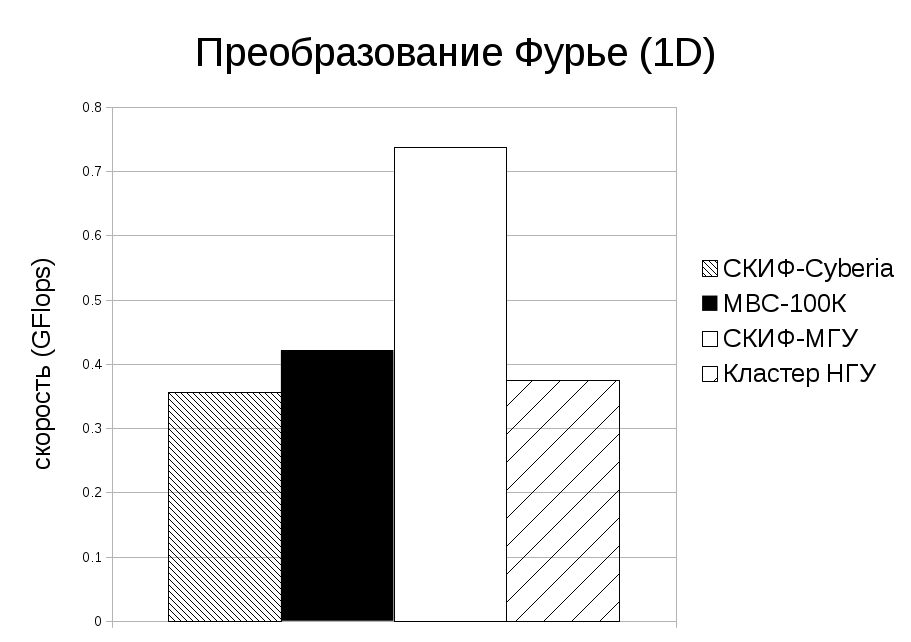
\includegraphics[height=7cm,keepaspectratio]{images/processor_FLOPS.png}
	\end{center}
	\caption{Производительность процессоров Intel Xeon, измеренная в ходе выполнения одномерного преобразования Фурье на некоторых кластерах. Размерность преобразования $N=64$. }
	\label{procs_flops}
\end{figure}

\textbf{Расчет производительности процессорных элементов на основе движения модельных частиц.}
Сравнительная производительность процессорных элементов некоторых из рассмотренных в диссертационной работе ВС выглядит как показано на рисунке  \ref{procs_flops_pic}:

\begin{figure}[htb]
	\begin{center}
		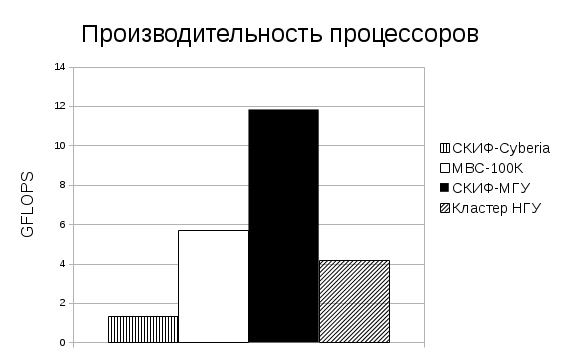
\includegraphics[height=7cm,keepaspectratio]{images/processor_FLOPS_PIC.png}
	\end{center}
	\caption{Производительность процессоров Intel Xeon, измеренная на основе времени вычисления движения модельных частиц. }
	\label{procs_flops_pic}
\end{figure} 

Расчет количества операций с плавающей точкой в секунду (FLOPS) при расчете движения модельных частиц $N_{PIC,FLOPS}$ производился следующим образом:
\begin{equation}
N_{PIC,FLOPS} = \frac{F_P\times N_P \times P_{core}}{\Delta t}
\label{PIC_FLOPS}
\end{equation}

здесь:
\begin{itemize}
	\item $F_P$ - количество операций на одну модельную частицу, $F_P = 440$;
	\item $N_P$ - количество модельных частиц на одно процессорное ядро (в рассмотренном случае $2.5\times 10^6$);  
	\item $P_{core}$ - количество ядер процессора;
	\item $\Delta t$  - длительность временного шага, сек.
\end{itemize}	

\begin{table}[ht]
	\caption{Производительность процессоров Intel Xeon, измеренная на основе времени вычисления движения модельных частиц.}
	\label{PIC_vs_PROC_RAM}
	\begin{tabular}{|c|c|c|c|c|c|}
		\hline
		&            &            &             &       \multicolumn{2}{|c|}{Производительность, GFLOPS} \\ \cline{5-6}  	
		Название ВС  & Процессор  &  $\Delta t$ &$P_{core}$ & Данные теста  &  \\
		&            &             &           & PIC-MANAS     & LU-разложение \\ \hline
		СКИФ-Cyberia & Xeon 5150  &  1.882      & 2     &  1.33          & 4.65    \\ \hline
		МВС-100К     & Xeon E5450 &  0.878      & 4     & 5.69           & 4.6     \\ \hline 
		СКИФ-МГУ     & Xeon E5472 &  0.423      & 4     & 11.83          & 2.37       \\ \hline     
		Кластер НГУ  & Xeon 5355  &  1.196      & 4     & 4.18           & 1.82       \\ \hline
	\end{tabular}	
\end{table}



\clearpage

\textbf{Расчет производительности коммуникационной сети.}
Разработана методика измерения быстродействия коммуникационной сети на основе анализа времени работы MPI-процедур, осуществляющих обмен граничными значениями между отдельными подобластями при решении уравнений Максвелла и при пересылке модельных частиц. В силу того, что при этом используются различные виды коммуникационных функций  - как блокирующие, так и не блокирующие, как парные, так и коллективные, при использовании эйлерово-лагранжевой декомпозиции - это позволяет набрать в течение одного расчета большую базу данных для получения знаний о структуре коммуникационной сети, времени прохождения сообщений в зависимоссти от размера, системных таймаутах и пр. 

\textbf{Оценка возможности выполнения крупномасштабных трехмерных расчетов.}
Проведены тестовые расчеты с целью определения эффективности распараллеливания и масштабируемости разработанных алгоритмов для моделирования взаимодействия электронного пучка с плазмой, а также с целью выяснения реальных возможностей суперЭВМ по проведению физических расчетов. Показано, что текущая версия программы позволяет проводить расчет на трехмерной сетке размером 350$^3$ узлов при 100 частицах в ячейке за 1 сутки на 10 ядрах суперкомпьютера «Ломоносов», или 42 млн.узлов. Эффективность распараллеливания составила 92 \% для максимального использованного числа ядер: 100 для кластера НГУ и 200 для кластера «Политехник».  

Целью расчетов  является ответ на вопрос, какие расчеты (т.е. какой размерности) могут быть проведены на доступных высокопроизводительных  ВС (ВВС), на каком количестве процессоров (или процессорных ядер) и за какое время. 
Для того, чтобы получить ответ на этот вопрос, было запущено большое количество тестовых расчетов. Эти тестовые расчеты носят предварительный характер, и проводятся также с целью выяснения реальных возможностей ВВС для проведения физически содержательных расчетов. 	Расчеты проводились на следующих ВВС: кластер СПбПУ “Политехник”, кластер НКС-1П (ССКЦ СО РАН), кластер НГУ,  кластер НИВЦ МГУ “Ломоносов”. 

\textbf{Формула для комплексной оценки ВС.}
Приведено обоснование формулы, на основании которой выносится оценка ВС по материалам проведенных тестов. При этом важно отметить, что оценка является не сравнительной - относительно других ВС, а абсолютной - с точки зрения математического моделирования. 

В частности, для того, чтобы параллельная ВС могла быть признана адаптированной к задачам математического моделирования, она должна соответствовать следующим требованиям:
\begin{enumerate}
	\item очень высокая производительность коммуникационной сети ($W_S$, формула \ref{Net_performance_peer} и $W_A$, формула \ref{Net_performance_collective} ), позволяющая пересылать все необходимые для расчета данные, не задерживая вычислений;
	
	\item относительно высокая производительность оперативной памяти ($W_{PIC,GB/sec}$, формула \ref{RAM_performance}), позволяющая эффективно использовать ресурсы процессоров, т.е. фактически совпадающая с производительностью процессора.  	
\end{enumerate}

Важно отметить, что названы относительные показатели, обеспечивающие возможность пересылать данные, без ущерба для скорости вычислений. Именно это и означает  комплексную пригодность ВС к решению задач математического моделирования.

В случае использования эйлерово-лагранжевой декомпозиции, т.е. если определены обе величины $W_S$ и $W_A$, будем использовать усредненную величину
\begin{equation}
W_{MPI} = \frac{W_S + W_A}{2}
\end{equation}
в случае только лишь эйлеровой или только лагранжевой декомпозиции, $W_{MPI}$ равна соотвественно, $W_S$ или $W_A$.

В итоге предлагается формула оценки $\xi$ в виде:
\begin{equation}
\xi = \frac{W_{MPI}} { W_{PIC,GB/sec}}, 
\label{complex_rating}
\end{equation}

\textbf{Сравнение с известными тестами производительности}
В этом разделе проведено сравнение с известными тестами производительности ВС, такими как HPL, HPCG. Сравнение показывает, что существует важное отличие разработанного теста от уже существующих, а именно значительно меньшая зависимость от правильного подбора конфигурации запуска. 


\underline{\textbf{Четвертая глава}} посвящена  
анализу масштабируемости, параллельной эффективности и ускорения параллельной ВС.

В четвертой главе предложена методика интегральной оценки тестируемой ВС с помощью измерения масштабируемости с расчетах по методу частиц в ячейках и определения на основе измерений возрастания потока данных в коммуникационной сети ВС.
%				На основе данных о пересылке модельных частиц измерена производительность коммуникационной сети ВС, при этом важно отметить преимущества использованного метода измерений: пересылка данных имеет высокую степень нерегулярности, а также большой объем, что означает проведение тестирования на большой нагрузке, и возможность широкого применения полученных таким образом данных.
%				Также предложена и апробирована методика определения фактически соседних (с точки зрения MPI) узлов ВС.  

%\subsubsection{Определение понятий эффективности, масштабируемости и ускорения}
%\textbf{Степаненко, книжка"высокопроизводительные вычисления", учебник Воеводина}




\textbf{Формулы для анализа данных о масштабируемости.}
\begin{equation}
\label{weak_eff}
\eta^{weak}_N = \frac{T^1(1)}{T^N(N)}
\end{equation}
здесь $T^K(N)$ обозначает время счета задачи с характерной размерностью $K$ при использовании $N$ процессоров.
это время состоит из двух основных частей:
\begin{itemize}
	\item собственно времени счета $T^K_{P}(N)$;
	\item времени коммуникаций $T^K_C(N)$;
\end{itemize}
Таким образом,
\begin{equation}
\label{weak_eff_detailed}
\eta^{weak}_N = \frac{T^1(1)}{T^N_{P}(N)+T^N_C(N)}
\end{equation}
при выполнении вычислений одновременно на однотипных процессорах
можно считать, что $T^1(1) = T^N_C(N)$, таким образом формула
\ref{weak_eff_detailed} приводится к виду:
\begin{equation}
\label{weak_eff_detailed-time}
\eta^{weak}_N = \frac{1}{1+ \frac{T^N_{C}(N)}{T^1(1)}}.
\end{equation}
Это означает, что при известном времени расчета задачи на одном процессоре можно восстановить время коммуникаций по эффективности в слабом смысле:
\begin{equation}
\label{comm_time_from_efficiency}
T^N_{C}(N) = T^1(1) \left(\frac{1}{\eta^{weak}_N} - 1\right)
\end{equation}
далее время коммуникаций может быть источником для вычисления производительности коммуникационной сети при известном объеме пересылок.

Приведены различные используемые варианты этих определений, перечислены факторы, влияющие на  значения этих величин для конкретной ВС, а именно скорость обмена данными и структура коммуникационной сети ВВС, алгоритмы реализации MPI-процедур, в особенности коллективных, настройки коммуникационной системы (таймауты, размер системных буферов, и др.).
%\textbf{написать формулы} 
%\textbf{привести формулы из статьи в СибЖВМ}
Для последующего анализа измеренного времени работы метода частиц в ячейках на параллельной ВС, и для прояснения зависимости этого времени от параметров расчета можно привести следующую схематическую формулу для длительности одного временного шага:

\begin{equation}
\label{PIC-timestep}
T=T_{F} \left ( \frac{N_x N_y N_z }{P_E}\right )+ T_{F,S}\left (N_y N_z\right ) + T_P\left(\frac{N_p}{P_E\times P_L}\right) +T_{P,S}\left (\frac{N_p*T_p}{P_E\times P_L}\right)
\end{equation}

здесь $T_{F}$ - время вычисления электромагнитного поля, $N_x, N_y, N_z$ - размер расчетной сетки соответственно, по координатам $X$ $Y$ и $Z$, $P_E$ - количество процессоров для эйлеровой декомпозиции, т.е. для разделения расчетной области на подобласти, $T_{F,S}$ - время, затрачиваемое на пересылку граничных значений полей и токов между подобластями, которое зависит только от $N_y$ и $N_z$ в силу того что на данный момент используется одномерная декомпозиция,  $T_P$ - время расчета движения частиц, $P_L$ - количество процессов (или потоков) для лагранжевой декомпозиции, т.е. для дополнительного разделения частиц подобласти на группы, вычисляемые на отдельных ядрах, $T_{P,S}$ - время, затрачиваемое на пересылку модельных частиц между подобластями.


\textbf{Вычисление характеристик коммуникационного оборудования ВС на основе измеренной масштабируемости метода частиц в ячейках.}

В этом разделе показаны измеренные характеристики масштабируемости параллельной программы, реализующей метод частиц в ячейках. Кроме того, сформулировано новое понятие \textbf{эффективного коммуникационного размера} ВС.

Результат измерения времени работы различных частей параллельного алгоритма на кластере НГУ показан в таблице \ref{NSU_itac}. Рост времени счета связан с тем, что размер сетки и количество частиц увеличивалось пропорционально количеству ядер.

\begin{table}[ht]
	\begin{center}
		\caption{Время выполнения (в секундах) наиболее времяемких частей реализации метода частиц на кластере НГУ}
		\begin{tabular}{|c|c|c|c|}
			\hline
			&  100 ядер    & 400 ядер \\ \hline
			Время счета (без учета MPI)   &  1110.8      & 4524.4   \\ \hline
			Процедура MPI\_Allreduce      &  136.3       & 553.3    \\ \hline
			Процедура MPI\_Comm\_size &  1.5         &  5.9    \\ \hline
			Процедура MPI\_Comm\_rank &  0.08        &  0.53            \\
			Процедура MPI\_Finalize   &  0.028        &  0.11  \\ \hline
			
		\end{tabular}
		\label{NSU_itac}
	\end{center}
\end{table}




Далее приведены фактически измеренные на различных высокопроизводительных ВС графики масштабируемости и параллельной эффективности и на основе этих данных проведен анализ коммуникационной сети рассматриваемых ВС, в частности, для МВС-100К, рис. \ref{eff2}. Кроме того, сформулировано новое понятие \textbf{эффективного коммуникационного размера} ВС.
 




Здесь мы подходим к решению одного из основных для всей диссертационной работы в целом - а именно вопроса о том, что расчет по методу частиц может прояснить в отношении ВС на которой он выполнялся. Для этого определим новую характеристику ВС:

\underline{\textbf{Определение}}: Эффективный коммуникационный размер ВС - максимальное количество процессоров, которое может быть в рамках данной ВС эффективно использовано для решения одной задачи.  

<<Эффективно>> в данном случае означает без существенного падения пропускной способности коммуникационной сети на MPI-пересылках при увеличении количества используемых узлов. За существенное падение в данной работы принято падение более чем в $e$ раз, при том, что безусловно, это не единственно возможный выбор. 

Особую важность представляет вопрос о коммуникационной связности ВС, т.е о том, до какой степени она способна функционировать как целое для решения одной большой задачи. Для решения этого вопроса предлагается перейти от масштабируемости как характеристики программы для решения задачи к анализу графика изменения производительности коммуникационной сети, полученного на основе данных о масштабируемости. Далее необходимо тем или иным способом выделить на этом рисунке участок с большими значениями производительности коммуникационной сети.
Один из возможных вариантов показан на рисунке \ref{scale_W_A_exp}, где показана аппроксимация этой зависимости гауссоидой. Далее дисперсия этой кривой (126) суммируется с начальной точкой (100), и полученное значение (226) и является эффективным коммуникационным размером данной ВС. Т.е. в данном случае эффективный коммуникационный размер - это количество процессоров, для которого производительность коммуникационной сети падает не более чем в $e$ раз по сравнению с максимальной.


\begin{figure}[h]
	
	
	\begin{center}
		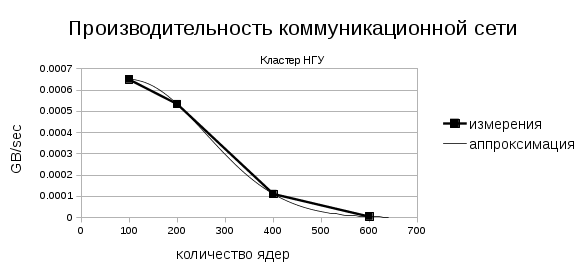
\includegraphics[height=5cm,keepaspectratio]{images/scaleNSU_exp_fit.png}
		\caption{
			Производительность коммуникационной сети для коллективных пересылок (величина $W_A$, формула \ref{Net_performance_collective}). 
		}
		\label{scale_W_A_exp}
	\end{center} 
\end{figure}

Далее вычислим эту же величину для двух наиболее характерных примеров зависимости эффективности в слабом смысле от числа процессорных ядер, представленных в диссертационной работе: для МВС-100К - сравнительно небольшая эффективность для большой разнородной ВС и для раздела ВВС <<Ломоносов>>, оснащенного GPU - очень высокая эффективность для однородной и компактной ВС. 

Напомним формулу для производительности коммуникационной сети ($W_A$, формула \ref{Net_performance_collective}):
$$
W_A = \frac{1}{P_{SUB}}\frac{N_X\times N_Y \times N_Z \times 24}{T_A}
$$
здесь:
\begin{itemize}
	\item $N_X, N_Y, N_Z$ - количество узлов сетки по X,Y и Z соответственно;
	\item $P_{SUB}$ - количество подобластей (если используется эйлерова декомпозиция)
	\item $T_{A}$ - длительность операции MPI\_Allreduce (суммирование токов по всей области), сек.
	\item множитель 24 появляется в силу того, что каждый элемент массива при двойной точности имеет размер 8, и таких массивов 3 (по одному для каждой из компонент тока).
\end{itemize}	

Для расчета раздела ВВС <<Ломоносов>>, оснащенного GPU, $N_X = 102, N_Y = 6, N_Z = 6, P_{SUB}  = 1$

 Эффективный коммуникационный размер для вычислительной системы  <<Ломоносов>> равен 239 (рисунок \ref{scale_W_A_Lomonosov}).


\begin{figure}[h]
	
	
	\begin{center}
		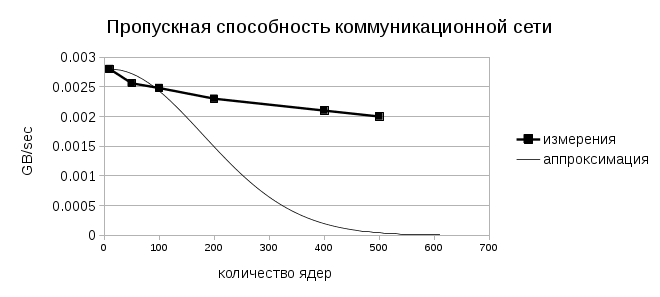
\includegraphics[height=5cm,keepaspectratio]{images/W_A_Lomonosov_Gauss.png}
		\caption{
			Производительность коммуникационной сети для коллективных пересылок (величина $W_A$, формула \ref{Net_performance_collective}). Расчет на сетке $100 \times 6 \times 6$ узла на <<Ломоносов>>, раздел с GPU. 
		}
		\label{scale_W_A_Lomonosov}
	\end{center} 
\end{figure}




\textbf{Анализ масштабируемости как интегральной характеристики ВС.}
Во втором разделе приведены фактически измеренные на различных высокопроизводительных ВС графики масштабируемости и параллельной эффективности и на основе этих данных проведен анлиз коммуникационной сети данных ВС, в частности, для МВС-100К, рис. \ref{eff2}. 

\begin{figure}[h]
	\begin{center}
		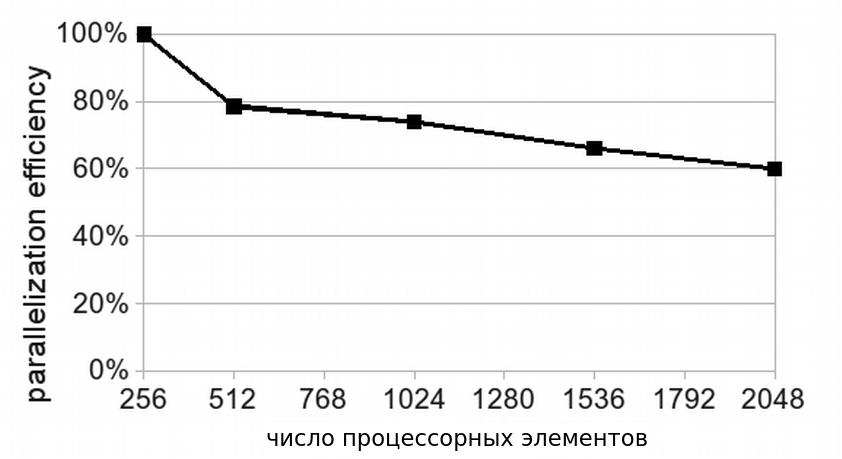
\includegraphics[height=5cm,keepaspectratio]{images/eff_weak_JSCC.png}
		\caption{
			Эффективность распараллеливания в слабом смысле, для МВС-100К, МСЦ РАН.
		}
		\label{eff2}
	\end{center} 
\end{figure}

Возможность проведения анализа коммуникационной сети с помощью расчетов по методу частиц в ячейках основана на известной информации о количестве пересылаемых данных и о виртуальной топологии, используемой в программе.

Размер данных, перемещаемых между двумя соседними MPI-процессами равен $144 \times N_y N_z  $ байт. При этом в идеальном случае, когда соседние MPI-процессы находятся на соседних узлах, коммуникации происходят только между соседними узлами, и поток данных в системе в целом не возрастает с ростом количества используемых в расчете узлов.

В частности, в расчете показанном на рис. \ref{eff2} использована эйлерова декомпозиция. Это означает, что используются только парные пересылки MPI, коллективные пересылки не используются, и поток данных через коммуникационную систему ВС в целом возрастать не должен. Если, тем не менее, он возрастает, что видно на рис. \ref{eff2} в виде снижения эффективности распараллеливания, то это может (при отсутствии коллективных операций) означать, что соседние с точки зрения MPI процессы находятся на физически удаленных друг от друга узлах параллельной ВС.

Обозначая $k_{||}$ зависимость коэффициента при времени пересылок граничных условий от количества процессоров в формуле \ref{PIC-timestep}, так что 
\begin{equation}
T_{F,S} = k_{||} (P_E) \frac{N_y N_z}{P_E}
\end{equation} 
и подставляя формулу (\ref{PIC-timestep}) в (\ref{weak_eff}), рассматривая только лишь время расчета и пересылок электромагнитного поля, можно получить 
\begin{equation}
k_{||} (P_E) = \frac{1}{\eta^{weak}(P_E)} - 1
\end{equation}	  
Таким образом величина $k_{||} (P_E)$  - \textbf{степень нелинейности} коммуникационной структуры параллельной ВС. Фактически она представляет собой отклонение от линейной функции для зависимости времени пересылок от количества процессоров. Он показывает предел возрастания потока данных через коммуникационную структуру ВС при увеличении количества процессоров, используемых в расчете. Эта величина характеризует, в какой степени при передаче информации между соседними процессами в MPI используются узлы параллельной ВС, не являющиеся ближайшими соседями. В силу того, что на значение эффективности оказывает влияние не только свойства оборудования, но и особенности реализации MPI, возникает необходимость разделить эти факторы. Это достигается с помощью привязки процессоров к узлам. 

В итоге, таким образом определенная  величина $k_{||} $ может быть использована как характеристика параллельной ВС, показывающая реально достижимую с помощью данной ВС эффективность и масштабируемость   

\textbf{Оценки параллельной масштабируемости на основе измерений времени прохождения сообщений.}
В этом разделе описано решение задачи об определении соседства процессов по реальным узлам. Это исключительно важно для производительности реальных задач, чтобы виртуально близкие (т.е. по номеру MPI-процесса) процессы исполнялись бы на соседних узлах многопроцессорной ВС. Для этого проводится обмен сообщениями между узлами, выделенными 
для исполнения программы по топологии полного графа, и проводится анализ времени прохождения сообщений.  

Следует отметить, что такого этапа, с обменом сообщениями между всеми процессами в рамках метода частиц нет, поэтому, такой анализ проводится предварительно, перед запуском основной части программы.



Узлы с минимальным временем считаются близкими, т.е. выясняется фактическая топология ВС. Это сопоставляется с известной информацией о размещении процессов по узлам.	Для повышения производительности приложения в дальнейшем целесообразно передвинуть соседние процессы на те узлы, где по факту меньше задержка по коммуникациям.

%	\textbf{картинку из стьатьи все-со-всеми, (с Политеха)}. 
%	1.измерение всех видов MPI-коммуникаций, сравнение одного с другим (Send, Isend, Bsend) - и увязатиь это с алгоритмом
%	2. варьирование размера сообщений и пр. параметров

%материал статьи НГУ ИТ  с более аакуратным анализом


\textbf{Определение зависимости масштабируемости от наличия и типа ускорителей вычислений.}

Проведено тестирование масштабируемости программы на ВВС, оснащенных различными типами ускорителей вычислений, в частности на кластере RSC Petastream в МСЦ РАН, результат показан на рис. \ref{phi100}. Видно, что в целом программа хорошо масштабируется.

\begin{figure}[htb]
	\begin{center}
		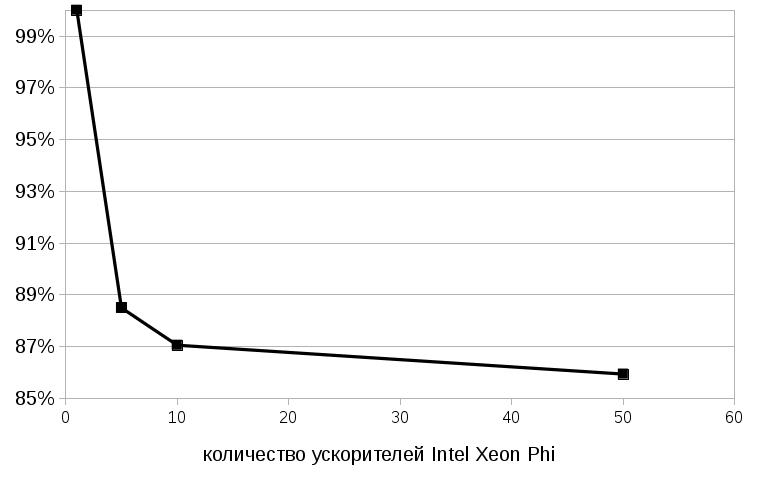
\includegraphics[height=5cm,keepaspectratio]{images/petastream_phi100.jpg}
	\end{center}
	\caption{Эффективность распараллеливания в слабом смысле с использованием Intel Xeon Phi. Расчет проведен на суперкомпьютере RSC Petastream, МСЦ РАН.}
	\label{phi100}
\end{figure}

Также было выполнено распалаллеливание на мелкозернистом уровне: по отдельным частицам в рамках ячейки: отдельные вычислительные потоки назначаются для счета траекторий отдельных частиц. Это было выполнено с помощью технологии CUDA для графических ускорителей (GPU) и с помощью технологии OpenMP для ускорителей Intel Xeon Phi. Программа PIC-MANAS может быть скомпилирована как для одного типа ускорителей (GPU), так и для другого (Intel Xeon Phi). Это достигается с помощью процедурных переменных и директив условной компиляции. 

Программа протестирована на кластере НКС-30Т (ИВМиМГ СО РАН), графические ускорители Nvidia Tesla M2090 (до 10) и Nvidia Kepler K40 и на суперЭВМ «Ломоносов»  (до 500 Nvidia Tesla C2070). Средняя продолжительность одного временного шага 0.01 секунды для  Nvidia Kepler K40 и 0.13 секунды для  Intel Xeon Phi (сетка $250\times250$, 100 модельных частиц в ячейке).



\textbf{Сравнение с известными тестами производительности}
В этом разделе проведено сравнение с известными тестами производительности ВС, такими как IMB. Сравнение показывает, что существует важное отличие разработанного теста от уже существующих, а именно значительно меньшая зависимость от правильного подбора конфигурации запуска.  

\underline{\textbf{Пятая глава}} посвящена 
анализу производительности узлов мультиархитектурной ВС.
В этой главе описаны методы, позволяющие определять скорость счета на ускорителях вычислений и скорость перемещения данных между ускорителем вычислений и хост-машиной, а также давать прогнозы о скорости счета нереализованных еще алгоритмов на тестируемой ВС.

Кроме того, предожена методика оценки качества узлов мультиархитектурной ВС на основе графических ( или других) ускорителей, при этом качество понимается как сбалнсированность средней оценочной скорости счета на ускорителе и скорости пермещения данныхмежду ускоритлем и хостом. 

\textbf{Анализ производительности узлов с графическмим ускорителями.}
редставлены результаты анализа производительности узлов с графическими ускорителями на основе измерения времени расчета движения модельных частиц, часть из которых показана в таблице \ref{PerfGPU}.

\begin{table}[ht]
	\begin{center}
		\caption{Характеристики выполнения основных частей реализации метода частиц на современных GPU}
		\begin{tabular}{|c|c|c|c|}
			\hline
			Название GPU                &  Tesla K80   & Tesla P100 \\ \hline
			Расчет электрического поля  &  25.3 мкс    &  16.059    \\ \hline
			Сдвиг частиц                &  348 мкс     &  338.16    \\ \hline
			Скорость копирования        &              &            \\
			частиц с хоста на GPU       & 4.92 ГБ/сек. &8.166 ГБ/сек.  \\ \hline
		\end{tabular}
		\label{PerfGPU}
	\end{center}
\end{table}

Основной вопрос данного раздела, как и всей работы - что можно узнать о данной ВС путем запуска программы, реализующей метод частиц в ячейках? В отличие от 	большинства других разделов информация о характеристиках оборудования в данном случае доступна через стандартный интерфейс, соответственно фактически измеренную скорость счета и скорость пересылки данных между хостом и GPU можно сравнивать с номинальными показателями.

Производительность GPU во флопсах также определяется по формуле (\ref{PIC_FLOPS}).

Важнейшей интегральной характеристикой ВС, оснащенной графическими ускорителями, является возможность их полноценно использовать. Эта возможность
может быть измерена с помощью сопоставления вычисленной скорости счета и скорости пересылок данных между хостом и GPU с использованием переводного множителя $k_{f2b}$. 
\begin{equation}
\label{kf2b}
k_{f2b} = 440/576 = 0.86
\end{equation}

Этот множитель отражает принципиальную возможность переслать необходимые данные с GPU на хост и далее по коммуникационной сети ВС на соседние узлы раньше, чем они понадобятся для счета на соседнем узле, и таким образом счет может продолжать без задержек, вызванных комммуникациями.

Вместе с тем вопрос, который наиболее часто задают специалисты по математическому моделированию применительно к мультиархитектурной ВС, оснащенной графическими ускорителями - это возможность \textit{эффективной} реализации конкретного вычислительного алгоритма на данной мультиархитектурной ВС.
Для ответа на данный вопрос предлагается интерполяционная формула:
\begin{equation}
v_{pre} = v_{PIC} k + (1-k) v_{B,E}
\end{equation} 
здесь $ v_{pre}$ - оценка скорости вычислений на GPU для рассматриваемого алгоритма, $v_{PIC}$ - скорость вычислений с на этапе сдвига модельных частиц, $v_{B,E}$ - на этапе расчета электромагнитного поля, а $k$ - интерполяционный множитель, получаемый из следующих соображений.

Как уже говорилось выше, большинство численных методов используемых в математическом моделировании находятся в промежуточном положении по отношению к используемым в методе частиц в ячейках алгоритму вычисления поля и алгоритму расчета движения частиц по следующим показателям:
\begin{itemize}
	\item вычислительной интенсивности (равномерное распределение вычислительно сложных фрагментов по тексту или отдельные высоконагруженные участки);
	\item характеру доступа к оперативной памяти (регулярный или нерегулярный);
	\item объему используемых данных (большой или маленький).
\end{itemize}
Ориентировочное распределение вычислительных алгоритмов по рассмотренным показателям и соответствующие значения коэффициента $k$ показаны в таблице 


\begin{table}[ht]
	\begin{center}
		\caption{Определение интерполяционного коэффициента для некоторых типов вычислительных алгоритмов}
		\begin{tabular}{|c|c|c|c|c|}
			%	        &   &  &  & k \\ \hline
			\hline
			Вычислительный    & Интенсивность &  Доступ к           & Объем  & $k$  \\ 
			алгоритм          &               &  оперативной  & данных &  \\
			&               &  памяти       &        &  \\ \hline
			Расчет движения   &  низкая       & нерегулярный        & большой & 1.0 \\ 
			модельных частиц  &               &                     &          & \\\hline
			Метод Монте-Карло &  низкая       & нерегулярный        & средний & 0.9 \\ \hline
			Метод SPH         &  низкая       & нерегулярный        & небольшой & 0.6 \\ \hline	Метод             &  высокая      & нерегулярный        & большой & 0.5  \\
			конечных элементов &          &              &         & \\ \hline
			Конечно-разностные &  высокая  & регулярный & большой & 0.2 \\ 		
			схемы (явные)      &           &            &         &     \\\hline
			Конечно-разностные &  высокая  & регулярный & большой & 0.1 \\ 		
			схемы (явные)-2    &           &            &         &     \\\hline
			Вычисление         &  высокая  & регулярный & большой & 0.0 \\ 		
			электромагнитного поля      &           &            &         &     \\\hline
			
			
		\end{tabular} 
		\label{tab-interp-koef}              
	\end{center}
\end{table}


\textbf{Механизм реализации переносимой программы}

Технология переноса программ численного моделирования с GPU на Intel Xeon Phi
будет показана на примере программы для моделирования динамики плазмы методом частиц в ячейках.

Вначале необходимо ответить на вопрос, для чего нужна такая методика?

Во-первых, необходимо иметь возможность использовать наиболее мощные гибридные суперЭВМ, а такие сейчас строятся (в том числе) на базе Intel Xeon Phi. Во-вторых, в
докладе А.О.Лациса “Что же делать с этим многообразием суперкомпьютерных миров?” на конференции <<Научный сервис в сети Интернет-2014>> \cite{Lacis2014} была предложена методика создания единого переносимого программного обеспечения для решения вычислительных задач, которое могло бы использоваться на многих суперкомпьтерных архитектурах. Эта методика основана на использовании библиотеки BLAS, которая так или иначе существует на всех машинах.


С точки зрения создания универсальной программы-теста важно, чтобы тестирование всех типов ВС происходило на основе строго одного и того же текста программы. Поэтому рассматривается вопрос именно о переносе, а не о создании аналогичного приложения для другой архитектуры. 

%Отднльно рассматривается вопрос о скорости подкачки данных к мультипроцессоорам GPU, т.е. производительность шины памяти, а также скорость загрузки данных из памяти хоста в память GPU. \textbf{таблица из статьи Булл и рассуждения}, вывод о качестве GPU и особ- \textbf{о качестве соединения} 

\textbf{Анализ производительности узлов с многоядерными процессорами и ускорителями вычислений.} 
Представлены результаты анализа производительности узлов с многоядерными процессорами разных типов и ускорителями вычислений, построенными по технологии, совместимой с x86 (Intel Xeon Phi различных поколений).

Основные вопросы те же, что и в разделе, посвященном графическим ускорителям: возможность полноценного использования вычислительной мощности 
ускорителей типа Intel Phi без задержек на перемещение данных и возможность эффективной реализации вычислительных алгоритмов на параллельной ВС, оснащенной ускорителями такого типа. Можно привести таблицу, аналогичную \ref{tab-interp-koef} с той поправкой, что эффективность многопоточного доступа к памяти на Intel Phi несколько ниже, поэтому значения интерполяционого коэффициента будут меньше для алгоритмов, использующих большой объем памяти.


В \underline{\textbf{заключении}} приведены основные результаты работы, которые заключаются в следующем:
%% Согласно ГОСТ Р 7.0.11-2011:
%% 5.3.3 В заключении диссертации излагают итоги выполненного исследования, рекомендации, перспективы дальнейшей разработки темы.
%% 9.2.3 В заключении автореферата диссертации излагают итоги данного исследования, рекомендации и перспективы дальнейшей разработки темы.
%\begin{enumerate}
 В работе предложена и реализована оригинальная методика комплексного тестирования мультиархитектурных параллельных вычислительных систем, основанная на используемой в реальных расчетах программе для математического моделирования. а именно на реализации метода частиц в ячейках.
 
 Особенностями предложенной методики комплексного тестирования являются возможность определения для конкретной ВС абсолютной оценки, основанной на степени пригодности данной ВС для решения задач математического моделирования, метод измерения возрастания потока данных в коммуникационной сети ВС, а также оценка эффективности реализации вычислительных алгоритмов для мультиархитектурных ВС.
 
 \textbf{Рекомендации и перспективы дальнейшей разработки темы.}
 Основным направлением совершенствования разработанного теста является автоматическая выработка рекомедаций по оптимизации кода, охватывающих не только методом частиц в ячейках но и остальные наиболее часто используемые в математическом моделировании методы,  под конкретную протестированную ВС.
 
 Одним из наиболее важных вариантов дальнейшего развития программы-теста, созданного в диссертационной работе является перенос на не охваченные в текущем варианте платформы, такие как Android, процессоры архитектуры Sunway.
 
 Кроме того, необходимостью является апробация теста на крупных высокопроизводительных ВС мощностью более петафлопса, а также - возможно, после специальной адаптации схемы расчета движения частиц - на ВС векторной архитектуры.
 
 
 
 
 
  
 
 
%\end{enumerate}


%При использовании пакета \verb!biblatex! список публикаций автора по теме
%диссертации формируется в разделе <<\publications>>\ файла
%\verb!../common/characteristic.tex!  при помощи команды \verb!\nocite!

\ifdefmacro{\microtypesetup}{\microtypesetup{protrusion=false}}{} % не рекомендуется применять пакет микротипографики к автоматически генерируемому списку литературы
\ifnumequal{\value{bibliosel}}{0}{% Встроенная реализация с загрузкой файла через движок bibtex8
	\renewcommand{\bibname}{\large \authorbibtitle}
	\nocite{*}
	\insertbiblioauthor           % Подключаем Bib-базы
	%\insertbiblioother   % !!! bibtex не умеет работать с несколькими библиографиями !!!
}{% Реализация пакетом biblatex через движок biber
	\ifnumgreater{\value{usefootcite}}{0}{
		%  \nocite{*} % Невидимая цитата всех работ, позволит вывести все работы автора
		\insertbiblioauthorcited      % Вывод процитированных в автореферате работ автора
	}{
		\insertbiblioauthor           % Вывод всех работ автора
		%  \insertbiblioauthorgrouped    % Вывод всех работ автора, сгруппированных по источникам
		%  \insertbiblioauthorimportant  % Вывод наиболее значимых работ автора (определяется в файле characteristic во второй section)
		\insertbiblioother            % Вывод списка литературы, на которую ссылались в тексте автореферата
	}
}
\ifdefmacro{\microtypesetup}{\microtypesetup{protrusion=true}}{}
